\documentclass{article}

\usepackage[final]{neurips_2026}

\usepackage[utf8]{inputenc}
\usepackage[T1]{fontenc}
\usepackage{hyperref}
\usepackage{url}
\usepackage{booktabs}
\usepackage{amsfonts}
\usepackage{amsmath}
\usepackage{nicefrac}
\usepackage{microtype}
\usepackage{xcolor}
\usepackage{graphicx}
\usepackage{subcaption}

\graphicspath{{figures/}}

\title{Political affiliation classification from French legislative campaign manifestos (1973--1993)}

\author{%
  Maël Trémouille \\
  ENSAE Paris \\
  \texttt{mael.tremouille@ensae.fr} \\
  Code: \url{https://github.com/MaelTremouille/political-text-classification}
}

\begin{document}

\maketitle

\begin{abstract}
We investigate whether political affiliation can be predicted from the text of French legislative campaign manifestos (\textit{professions de foi}) spanning five elections between 1973 and 1993.
We work with 4{,}519 documents from the Archelec archive, extract party labels via regex pattern matching, and frame the task as a four-class classification problem over broad political families.
We compare a TF-IDF logistic regression baseline against a fine-tuned CamemBERT model.
The baseline achieves 84\% accuracy while CamemBERT only reaches 71\%, which suggests that simple word-level features are enough for this type of corpus.
We also look at inter-party semantic proximity using sentence-transformer embeddings, t-SNE, and cosine similarity.
\end{abstract}

%----------------------------------------------------------------------
\section{Introduction}
\label{sec:intro}
%----------------------------------------------------------------------

In France, \textit{professions de foi} are official campaign statements distributed to all registered voters before legislative elections. Because they follow a relatively standard format across parties and years, they form an interesting corpus for studying political discourse.

We ask the following question: \textbf{can we predict a candidate's political affiliation from the text alone, without any explicit party mention?} If so, what features distinguish each political family? And how do parties relate to one another in a semantic embedding space?

We use the Archelec corpus~\citep{archelec}, which contains digitized and OCR'd \textit{professions de foi} from French legislative elections held in 1973, 1978, 1981, 1988, and 1993. The OCR'd text files were obtained directly from the course repository\footnote{\url{https://gitlab.teklia.com/ckermorvant/arkindex\_archelec}}, so we did not have to perform any OCR processing. This twenty-year period covers significant changes in the French political landscape, from left-wing coalitions in the 1970s to alternations of power in the 1980s and 1990s.

Our approach is as follows. First, we build a labeled dataset by extracting party mentions from the text using regular expressions, then removing these mentions to prevent data leakage (Section~\ref{sec:data}) (\textit{i.e.} we did not want the model to cheat by learning to detect the name of the party in the text). Second, we compare a TF-IDF logistic regression baseline with a fine-tuned CamemBERT model~\citep{martin2020camembert} (Section~\ref{sec:models}). Third, we analyze inter-party distances through sentence-transformer embeddings (Section~\ref{sec:results}) to allow a visualization in a political 2D mapping. Implementation details are provided in Appendix~\ref{app:implementation}.

%----------------------------------------------------------------------
\section{Related work}
\label{sec:related}
%----------------------------------------------------------------------

\paragraph{Text-based political analysis.}
The idea of using text to analyze political positions is not new. \citet{laver2003extracting} proposed a method (Wordscores) that uses word frequencies to estimate party policy positions from political texts, by comparing each text to pre-scored reference documents. They applied it to party manifestos in Britain and Ireland. The Manifesto Project~\citep{volkens2013manifesto} took this further by building a large hand-coded database of party platforms across dozens of countries and decades, which is widely used in political science. More recently, \citet{rheault2020word} trained word embedding models augmented with party metadata on parliamentary debates from Britain, Canada, and the United States, showing that these representations can capture ideological differences between parties.

Our work is close to Laver et al. in that we also use text to infer political positioning, but we frame the problem differently: instead of estimating positions on a continuous scale, we classify documents into discrete political families. We also work with French \textit{professions de foi} rather than English-language manifestos, and compare a classical approach (TF-IDF) with a pretrained transformer model.

\paragraph{NLP for French political texts.}
Most of the work cited above focuses on English. Political NLP in French is less developed. The Archelec project~\citep{archelec} has made a large corpus of digitized \textit{professions de foi} publicly available, but the project itself focuses on digitization and OCR rather than on downstream NLP tasks like classification.

\paragraph{CamemBERT.}
CamemBERT~\citep{martin2020camembert} is a RoBERTa-based model pretrained on a large French web corpus (OSCAR). It has been shown to achieve good results on standard French NLP benchmarks, including named entity recognition, part-of-speech tagging, and text classification. Since our task is text classification in French, it was a natural model to try.

%----------------------------------------------------------------------
\section{Data}
\label{sec:data}
%----------------------------------------------------------------------

\subsection{Corpus description}

The Archelec corpus consists of scanned and OCR'd \textit{professions de foi} from French legislative elections. Each raw file corresponds to a single scanned page, following a naming convention that encodes metadata: election identifier, year, department code, constituency number, election round, and document type. It is then easy to build a database that reconstructs the whole documents using the available information.

We keep only \textit{professions de foi} (tagged \texttt{PF}), we delete ballots (\texttt{BV}) and OCR processing artifacts (\texttt{pdfmasterocr}). Multi-page documents belonging to the same candidate are concatenated in page order to reconstruct complete texts. After aggregation, the corpus contains 4{,}658 documents that cover five election years.

\subsection{Label extraction}
\label{sec:labels}

The corpus does not include structured party labels, but it seemed possible to directly extract them thanks to the normalized form of \textit{profession de foi}. We extract them from the text itself using a two-stage regex approach:

\begin{enumerate}
    \item \textbf{Full name patterns}: we search the entire text for explicit party names (e.g., \textit{Parti Communiste Fran\c{c}ais}, \textit{Rassemblement pour la R\'{e}publique}). Patterns handle OCR variants (accented and unaccented characters, variable spacing). They are ordered from most specific to least specific to avoid ambiguous matches (e.g., we search for \textit{Parti Socialiste Unifi\'{e}} before \textit{Parti Socialiste}, otherwise PSU texts would be mislabeled as PS).
    \item \textbf{Abbreviation patterns}: for remaining unlabeled documents, we search the first 1{,}000 characters for common acronyms (e.g., PS, RPR, UDF), restricting to the header area to limit false positives from opponents mentioned in the text body. It allowed us to narrow the proportion of unlabeled texts to about 2\%.
\end{enumerate}

This procedure labels 97.8\% of documents (4{,}557 out of 4{,}658). We identify 17 distinct party labels, which we group into five political families: \textit{Extr\^{e}me gauche} (LO, LCR), \textit{Gauche} (PCF\footnote{The PCF could arguably be classified as \textit{Extr\^{e}me gauche}. We place it in \textit{Gauche} because, during the 1973--1993 period, the PCF was part of the Union de la Gauche coalition with the PS and participated in government (1981--1984).}, PS, PSU, MRG), \textit{\'{E}cologistes} (Verts), \textit{Droite} (RPR, UDF, UDR, RI, and coalition labels), and \textit{Extr\^{e}me droite} (FN, PFN).

We do not take into account the \'{E}cologistes class (38 documents), which is too small for meaningful classification (we could not classify them well without decreasing the overall results too much). The final dataset contains \textbf{4{,}519 documents} over four political families.

\paragraph{Data leakage prevention.}
Since we aim to classify political affiliation from discourse content rather than explicit party names, we remove all party mentions from the text using the same regex patterns. This produces a cleaned text column used for all the models.

\subsection{Dataset statistics}


Table~\ref{tab:distribution} shows the distribution across political families and election years. The dataset is heavily imbalanced: Gauche represents 60\%
of documents, while Extr\^{e}me droite accounts for only 1.4\%. We initially worried that this was an artifact of our regex approach, but the imbalance has two real causes.  
\begin{table}[h]
  \caption{Number of labeled documents by political family and election year.}
  \label{tab:distribution}
  \centering
  \begin{tabular}{lccccc|c}
    \toprule
    Family & 1973 & 1978 & 1981 & 1988 & 1993 & Total \\
    \midrule
    Extr\^{e}me gauche & 274 & 473 & 178 & 0 & 241 & 1{,}166 \\
    Gauche              & 564 & 374 & 568 & 763 & 444 & 2{,}713 \\
    Droite              & 27  & 36  & 51  & 227 & 237 & 578 \\
    Extr\^{e}me droite  & 1   & 0   & 0   & 3   & 58  & 62 \\
    \midrule
    Total               & 866 & 883 & 797 & 993 & 980 & 4{,}519 \\
    \bottomrule
  \end{tabular}
\end{table}

First, our extraction method has an inherent bias: left-wing parties (especially PCF and LO) systematically state their party name in their \textit{professions de foi}, while right-wing candidates more often present themselves under coalition labels or without explicit party mention. But even if all unlabeled documents were right-wing, the imbalance would remain. The second reason could simply be that there were more left-wing candidates running in legislative elections during this period.

Looking at text length, we found large differences between families (Table~\ref{tab:lengths}). Extr\^{e}me gauche documents are by far the longest, with a mean of about 6{,}700 words, compared to roughly 1{,}100 for Droite. This is probably because LO and LCR candidates tend to write very detailed manifestos that go through many political topics, while right-wing candidates write shorter, more focused texts. Gauche is somewhere in between (mean around 2{,}300 words). This difference in length is important to keep in mind, because TF-IDF features will naturally accumulate more for longer documents, which could give the model additional signal beyond just vocabulary.

\begin{table}[h]
  \caption{Text length statistics (word count) by political family after party name removal.}
  \label{tab:lengths}
  \centering
  \begin{tabular}{lccc}
    \toprule
    Family & Mean & Median & Std \\
    \midrule
    Extr\^{e}me gauche & 6{,}681 & 6{,}382 & 2{,}378 \\
    Gauche              & 2{,}334 & 1{,}775 & 1{,}776 \\
    Extr\^{e}me droite  & 1{,}214 & 1{,}016 & 787 \\
    Droite              & 1{,}068 & 839   & 984 \\
    \bottomrule
  \end{tabular}
\end{table}

We split the data into train (70\%, 3{,}163 documents), validation (15\%, 678), and test (15\%, 678) using stratified sampling on the political family label.

%----------------------------------------------------------------------
\section{Models}
\label{sec:models}
%----------------------------------------------------------------------

We frame political affiliation prediction as a classification task with four classes. We train two models of different complexities.

\subsection{Baseline: TF-IDF + logistic regression}

TF-IDF (Term Frequency--Inverse Document Frequency) weighs each term by how frequent it is in a document relative to how common it is across the whole corpus. A word that appears often in one document but rarely elsewhere gets a high weight, while very common words (like ``de'' or ``les'') get a low weight.

We represent each document as a TF-IDF vector with up to 20{,}000 features, including unigrams and bigrams. We set a minimum document frequency of~3, meaning that a term must appear in at least 3~documents to be included; this filters out OCR artifacts, typos, and overly rare words that would add noise without predictive value.

We train a logistic regression classifier with L2 regularization and balanced class weights. The \texttt{balanced} option automatically adjusts the loss contribution of each class in inverse proportion to its frequency in the training set, which helps the model pay attention to minority classes like Extr\^{e}me droite (only 43 training examples).

This baseline has two main advantages: it is fast to train, and it sees the \emph{entire} document regardless of length, unlike transformer-based models which truncate inputs.

\subsection{CamemBERT fine-tuning}

CamemBERT~\citep{martin2020camembert} is a French language model based on the RoBERTa architecture, pretrained on a large French web corpus (OSCAR) using masked language modeling. It learns contextual word representations: the same word gets a different embedding depending on its surrounding context, unlike TF-IDF which treats each word independently.

We fine-tune \texttt{camembert-base} (110M parameters) for sequence classification. The model adds in the beginning of the sequence a special \texttt{[CLS]} token to the input. After passing through 12 layers of self-attention, this token's output vector acts as a fixed-size summary of the entire text. We add a linear classification layer on top of this vector to produce one score per class; the highest score is the predicted label. Input texts are tokenized with the SentencePiece tokenizer and truncated to a maximum of 512 tokens, which is a hard constraint of the model architecture.

To handle class imbalance, we use a weighted cross-entropy loss where each
class receives a weight inversely proportional to its frequency, following
the same logic as the balanced logistic regression. Note that at this stage
we had already removed the \'Ecologistes class, because giving it a very
high weight (to compensate for only 38 documents) was destabilizing the
training. We explored several training configurations (Table~\ref{tab:configs}),
varying the number of epochs and the use of a linear learning rate scheduler:
the learning rate starts at zero, increases linearly during the first 10\%
of training steps (warmup), then decreases back to zero. This helps avoid
large gradient updates early in training when the model has not yet adapted
to the task. Additional configurations that did not improve results are
detailed in Appendix~\ref{app:training}.

\begin{table}[h]
  \caption{CamemBERT training configurations and test accuracy.}
  \label{tab:configs}
  \centering
  \begin{tabular}{ccccc}
    \toprule
    Run & Epochs & Weighted loss & LR scheduler & Test accuracy \\
    \midrule
    1 & 3 & Yes & No  & 68\% \\
    2 & 5 & Yes & Yes & 71\% \\
    \bottomrule
  \end{tabular}
\end{table}

All runs use AdamW (a variant of the Adam algorithm) with a learning rate of $2 \times 10^{-5}$, weight decay of 0.01, and a batch size of 8. Training is performed on an Apple M-series GPU (MPS backend). We did not use external GPU resources since the dataset is small enough for training to run in a reasonable time on a laptop.

\subsection{Semantic mapping}

Beyond classification, we want to visualize how close or far parties are from each other in terms of discourse. The idea is to represent each document as a vector (an embedding), then compare these vectors to measure semantic proximity (and thus discourse proximity).

We first tried using the \texttt{[CLS]} vector from the pretrained CamemBERT base model (without fine-tuning), but this did not work: all pairwise cosine similarities exceeded 0.98, so every party looked identical (see Appendix~\ref{app:cls_failure}) meaning the model treated all discourses the same. The reason is that CamemBERT base was trained to predict masked words, not to produce embeddings that reflect meaning --- and because all \textit{professions de foi} share the same formal register, the \texttt{[CLS]} vectors just converge and give similar values.

We then switched to a sentence-transformer\footnote{\texttt{dangvantuan/sentence-camembert-large}, available at \url{https://huggingface.co/dangvantuan/sentence-camembert-large}}, which is built on CamemBERT-large but fine-tuned for semantic similarity . We use CamemBERT-large rather than base here because this sentence-transformer model is only available in a large version on Hugging Face, and since we do not fine-tune it, the larger size is not a problem. Instead of using the \texttt{[CLS]} token alone, it averages all token embeddings from the last layer (mean pooling) to produce one vector per document. The idea is that two texts about similar topics should end up with similar vectors, and texts about different topics should be far from one another. This gave us much more usable results.

Once we have embeddings for all documents, we compute mean vectors per party and per political family. To compare parties, we use cosine similarity, which measures how aligned two vectors are (1 = same direction, 0 = orthogonal). For visualization, we use t-SNE (t-distributed Stochastic Neighbor Embedding), which projects the high-dimensional vectors onto a 2D plane while trying to preserve local neighborhoods. t-SNE is good for spotting clusters but can distort global distances, so the plots should be read with some attention.

%----------------------------------------------------------------------
\section{Experiments and results}
\label{sec:results}
%----------------------------------------------------------------------

\subsection{Classification performance}

Table~\ref{tab:results} reports test set results for both models.

\begin{table}[h]
  \caption{Test set performance. TF-IDF outperforms CamemBERT across all metrics.}
  \label{tab:results}
  \centering
  \begin{tabular}{lccc}
    \toprule
    Model & Accuracy & Macro F1 & Weighted F1 \\
    \midrule
    TF-IDF + Logistic Regression & \textbf{0.84} & \textbf{0.80} & \textbf{0.85} \\
    CamemBERT (best, Run 2)     & 0.71          & 0.65          & 0.72 \\
    \bottomrule
  \end{tabular}
\end{table}

\paragraph{Per-class analysis.}
Table~\ref{tab:per_class} shows per-class F1 scores.

\begin{table}[h]
  \caption{Per-class F1 scores on the test set.}
  \label{tab:per_class}
  \centering
  \begin{tabular}{lcc}
    \toprule
    Family & TF-IDF + LR & CamemBERT \\
    \midrule
    Extr\^{e}me gauche & 0.96 & 0.73 \\
    Gauche              & 0.86 & 0.76 \\
    Droite              & 0.60 & 0.54 \\
    Extr\^{e}me droite  & 0.76 & 0.57 \\
    \bottomrule
  \end{tabular}
\end{table}

TF-IDF does better than CamemBERT on every class. The easiest family to classify is Extr\^{e}me gauche (F1 = 0.96) --- LO and LCR have a very recognizable vocabulary. Droite is the hardest (F1 = 0.60). To understand where errors come from, we look at the full confusion matrix (Table~\ref{tab:confusion}).

\begin{table}[h]
  \caption{Confusion matrix for TF-IDF + Logistic Regression on the test set. Rows are true labels, columns are predictions.}
  \label{tab:confusion}
  \centering
  \begin{tabular}{lcccc}
    \toprule
    & \textit{Droite} & \textit{Ext. droite} & \textit{Ext. gauche} & \textit{Gauche} \\
    \midrule
    Droite              & \textbf{70} & 4  & 1   & 12 \\
    Extr\^{e}me droite  & 1  & \textbf{8} & 0   & 0 \\
    Extr\^{e}me gauche  & 0  & 0  & \textbf{171} & 4 \\
    Gauche              & 76 & 0  & 10  & \textbf{321} \\
    \bottomrule
  \end{tabular}
\end{table}

The main source of error is clear: 76 Gauche documents get misclassified as Droite, and 12 Droite documents end up as Gauche. This is not really surprising --- once we remove party names, mainstream left and right candidates tend to talk about the same topics (employment, housing, education) using similar words. In contrast, Extr\^{e}me gauche is almost never confused with anything else (only 4 misclassified as Gauche out of 175).

Looking at precision and recall gives more insight. For Droite, the model has high recall (0.80) but low precision (0.48): it correctly finds most Droite documents, but it also wrongly labels many Gauche texts as Droite. This means the boundary between mainstream left and right discourse is genuinely blurry in these texts. For Extr\^{e}me gauche, both precision (0.94) and recall (0.98) are very high, which confirms that this family has a really distinctive way of writing.

\paragraph{What words drive the classification?}
To understand what the model actually learns, we looked at the logistic regression coefficients. Since we use a one-vs-rest scheme, the model trains one logistic regression per class, each with its own vector of 20{,}000 coefficients (one per TF-IDF feature). To predict a document's class, we compute the score from each of the four logistic regressions and take the argmax --- the class whose model gives the highest score wins. A high positive coefficient for a given word in a given class model means that the presence of this word pushes the score up for that class. So by sorting the coefficients of each model, we get the words that are the most ``useful'' for predicting each political family. The full top~20 for each class is given in Appendix~\ref{app:features}.

For \textit{Extr\^{e}me gauche}, the most discriminative feature is ``travailleurs'' (\textit{workers}). This is the typical vocabulary of LO and LCR manifestos, which consistently use class-struggle language. We also observe that many function words (``les'', ``de'', ``des'') appear with high coefficients for this class, which we think is partly an artifact of text length: since these documents are on average 6 times longer than Droite texts (Table~\ref{tab:lengths}), common French words end up with higher TF-IDF scores simply because they accumulate more.

For \textit{Droite}, we found features like ``notre'' (\textit{our}), ``solidarit\'{e}'' (\textit{solidarity}), and ``france unie'' (\textit{united France}), but also many date-related terms (``12 juin'', ``juin 1988'') and geographic names (``la r\'{e}union'', ``guadeloupe'', ``corse''). The presence of overseas department names is interesting --- it suggests that right-wing candidates in these departments are overrepresented in our labeled data, or that their discourse is distinctive enough to be picked up by the model.

For \textit{Extr\^{e}me droite}, ``le pen'' and ``fran\c{c}ais'' (\textit{French}) are among the strongest features. The name ``Le~Pen'' was not removed by our cleaning procedure since we only remove party names, not candidate names. This is a form of indirect leakage that we did not anticipate: FN candidates frequently mention their leader by name in their manifestos, so the model can partially rely on this.

For \textit{Gauche}, we notice that ``communiste'' and ``gauche'' appear as discriminative features. These words were not removed either, because our regex targets full party names (``Parti Communiste Fran\c{c}ais'') rather than individual words. Candidates who write ``je suis candidat communiste'' or ``candidat de gauche'' still leave these markers in the cleaned text. This is a limitation of our cleaning approach, and it probably helps the model more than it should.

Overall, the feature analysis shows that the classifier relies on a mix of genuinely political vocabulary, stylistic differences linked to text length, and some residual markers that our cleaning did not fully remove. The high performance on Extr\^{e}me gauche seems to be driven by both a distinctive militant vocabulary \textit{and} the much longer text length of these documents.

\paragraph{CamemBERT analysis.}
CamemBERT clearly overfits: the training loss goes down steadily (from 1.18 to 0.43 over 5 epochs) but validation accuracy stops improving after epoch 2, around 72\%. This is probably because 3{,}163 training examples is just not enough for a model with 110 million parameters, so it ends up memorizing the training data instead of learning general patterns. On top of that, \textit{professions de foi} tend to reuse the same party-specific keywords, so simple word counting already captures most of the signal; contextual understanding does not help much here. The 512-token truncation is another problem: since Extr\^{e}me gauche texts average 6{,}700 words but CamemBERT only sees the first 512 tokens (roughly 300--400 words), the model misses most of the document. TF-IDF does not have this constraint and can use the full text. And with only 43 Extr\^{e}me droite examples in the training set, even weighted loss cannot really compensate. In the end, a simple bag-of-words approach works better than a large pretrained model on this corpus, which is an interesting result in itself.

\subsection{Semantic mapping}
\label{sec:mapping}

Figure~\ref{fig:tsne} shows the t-SNE projection of all document embeddings, colored by political family. There is some left-right separation --- blue points (Droite) tend to be on one side, red points (Gauche, Extr\^{e}me gauche) on the other --- but the overlap in the middle is significant. The families are not clearly separated, which is consistent with what the classifier showed.

\begin{figure}[h]
  \centering
  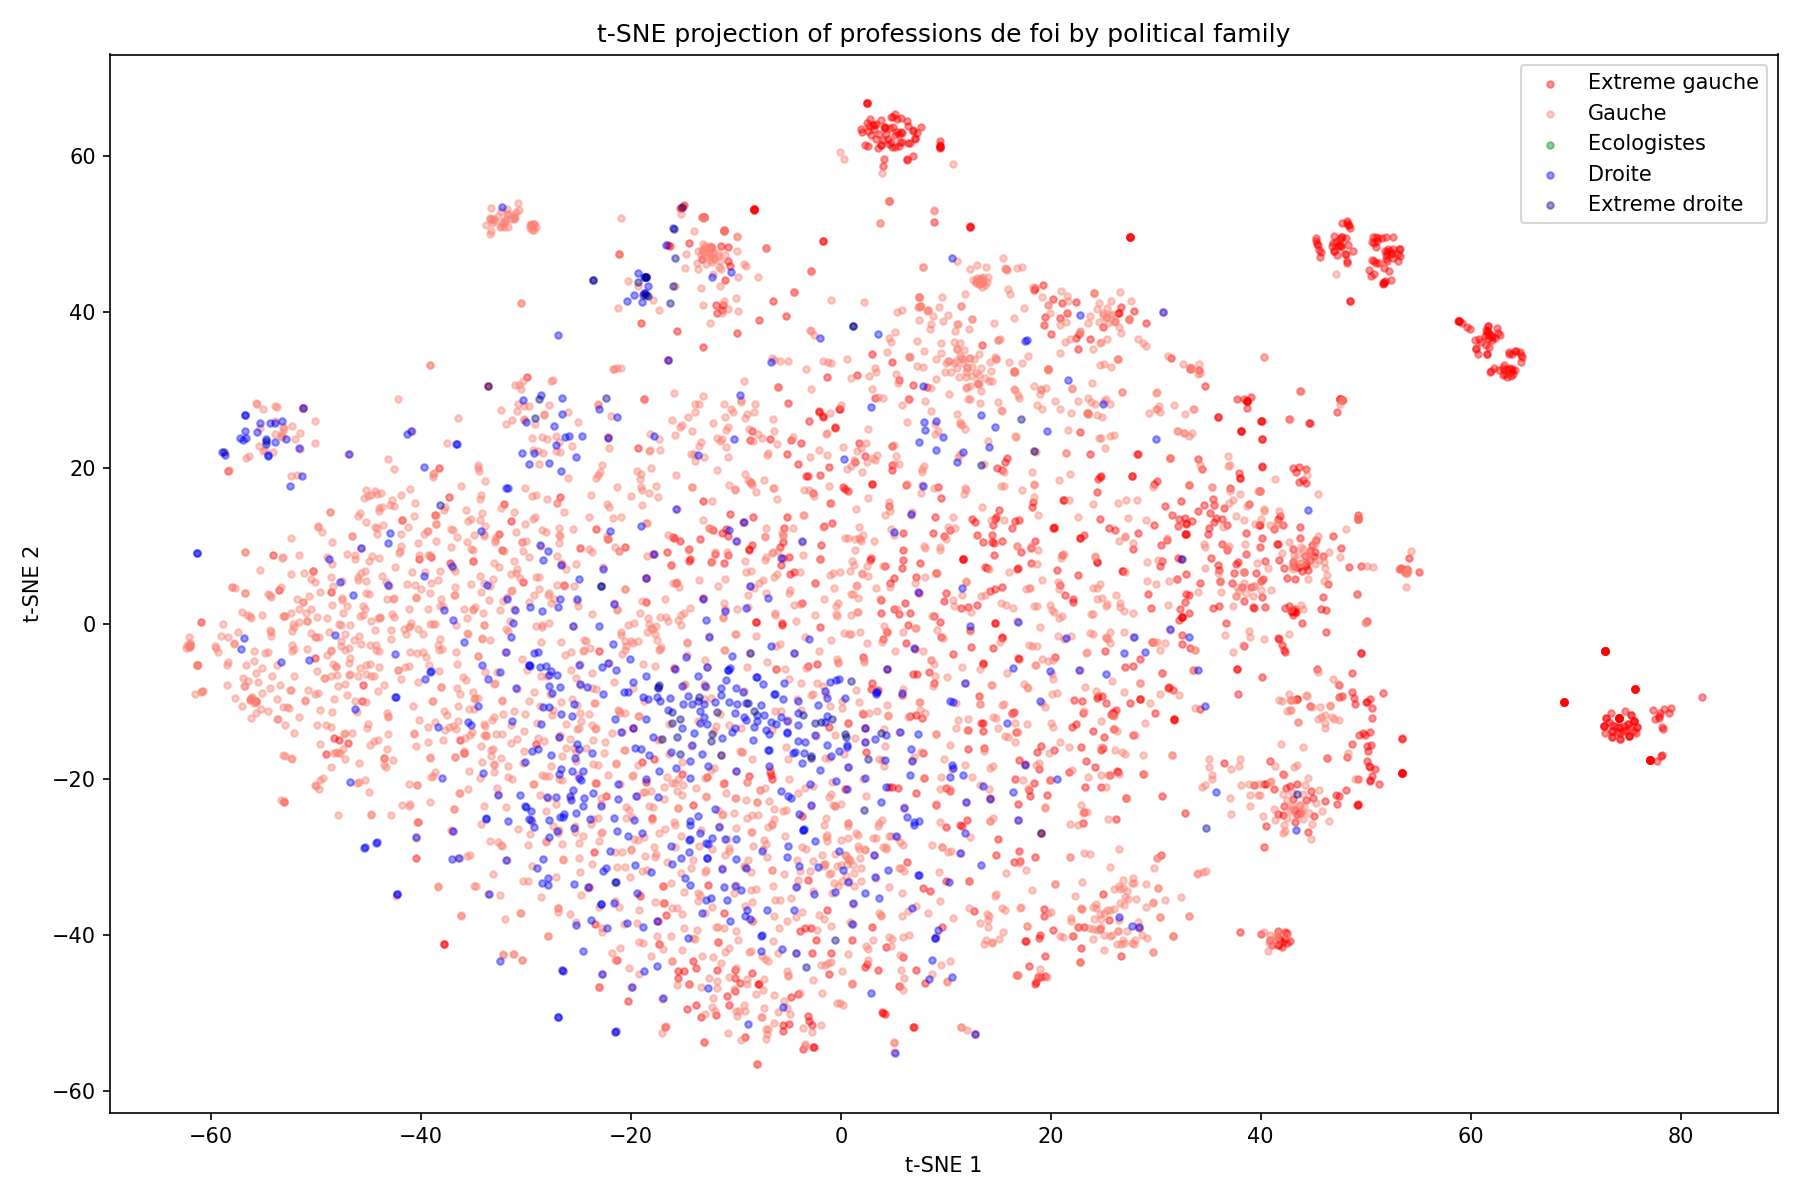
\includegraphics[width=0.9\linewidth]{tsne_by_family.png}
  \caption{t-SNE projection of document embeddings colored by political family. Partial left-right separation is visible but overlap is significant.}
  \label{fig:tsne}
\end{figure}

The cosine similarity heatmap (Figure~\ref{fig:cosine}) gives a more precise picture. Most party pairs have similarity above 0.90, which makes sense given that all \textit{professions de foi} use a similar formal style. The RPCR stands out clearly as an outlier (similarity around 0.70--0.78 with everyone else) --- it is a regionalist party from New Caledonia, so its discourse is about overseas territorial issues rather than metropolitan French politics. We can also see that LO and PSU are a bit less similar to right-wing parties than PS or MRG, which is expected given their more radical positioning.

\begin{figure}[h]
  \centering
  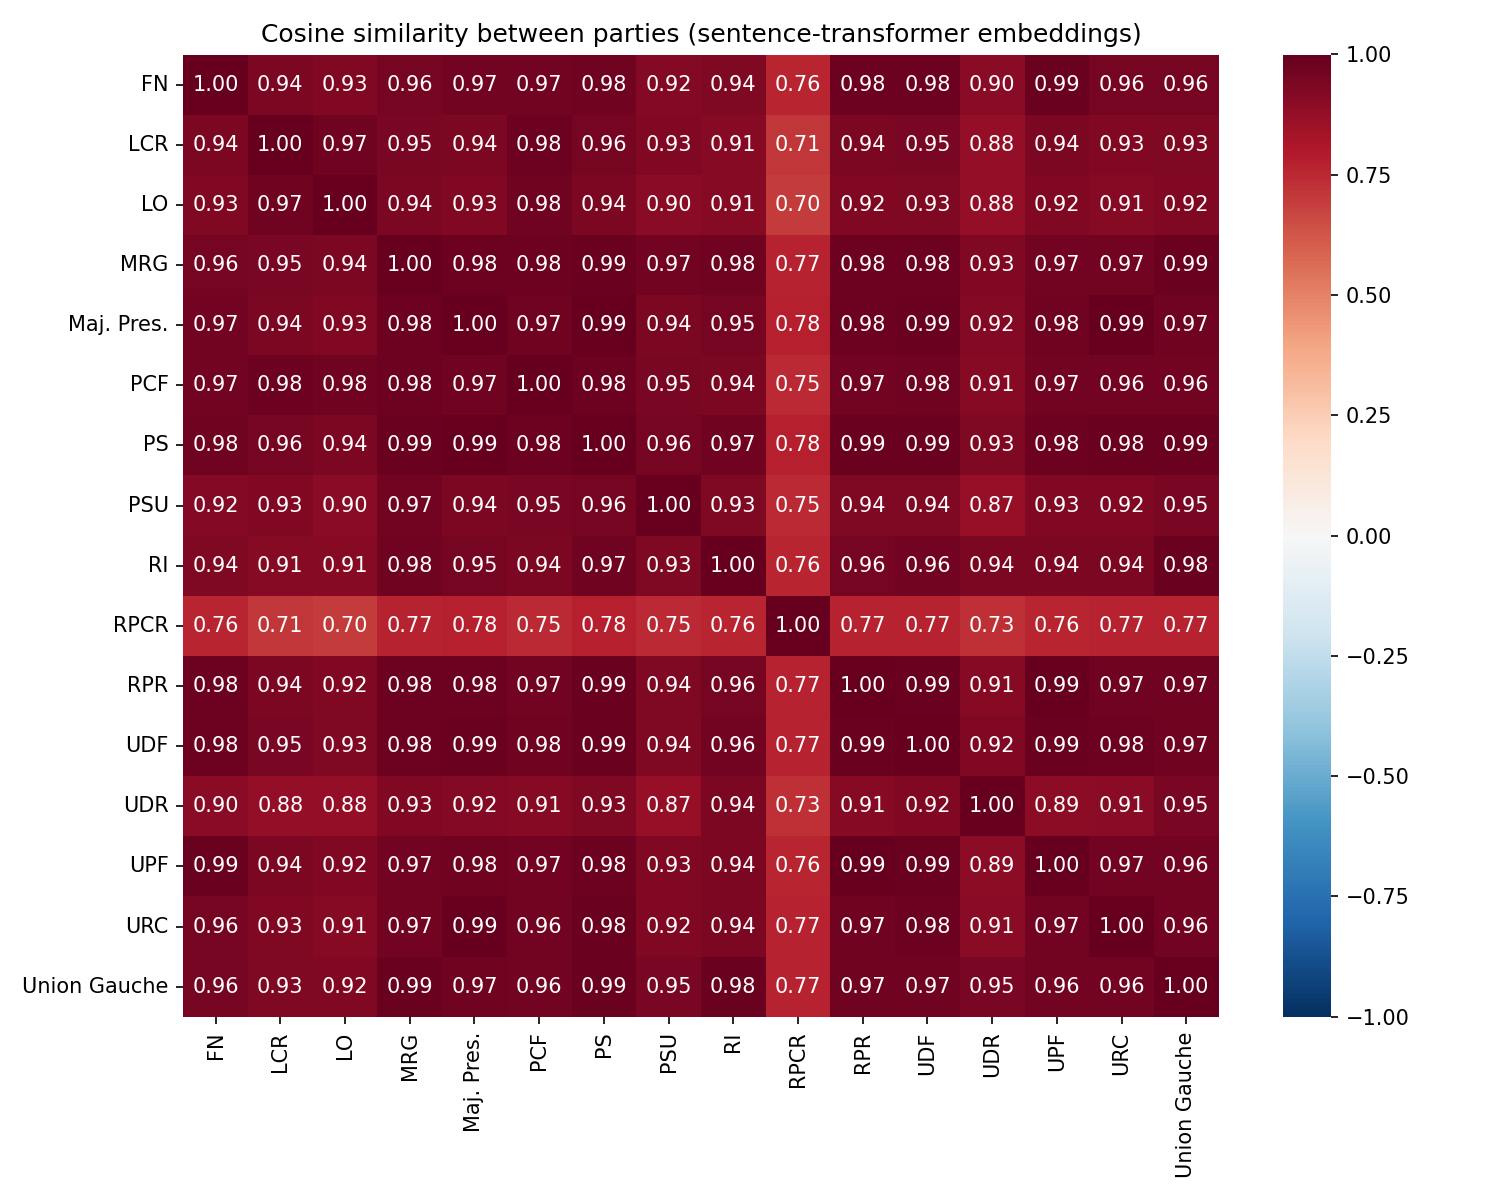
\includegraphics[width=0.85\linewidth]{cosine_similarity_parties.png}
  \caption{Cosine similarity between mean party embeddings (sentence-transformer). The RPCR stands out as an outlier; other parties cluster above 0.88.}
  \label{fig:cosine}
\end{figure}

We also tried to look at how discourse evolves over the years. For this, we compute a mean embedding for each (family, election year) pair --- so for example, ``Gau 1973'' represents the average of all Gauche documents from 1973 --- and project everything with t-SNE (Figure~\ref{fig:temporal}). There are only 18 points on this plot, so we cannot draw strong conclusions. What we can see is that points from the same family do not always end up close together: Droite in 1973 and Droite in 1993 can be quite far apart, suggesting that the way parties talk changes over the years.

\begin{figure}[h]
  \centering
  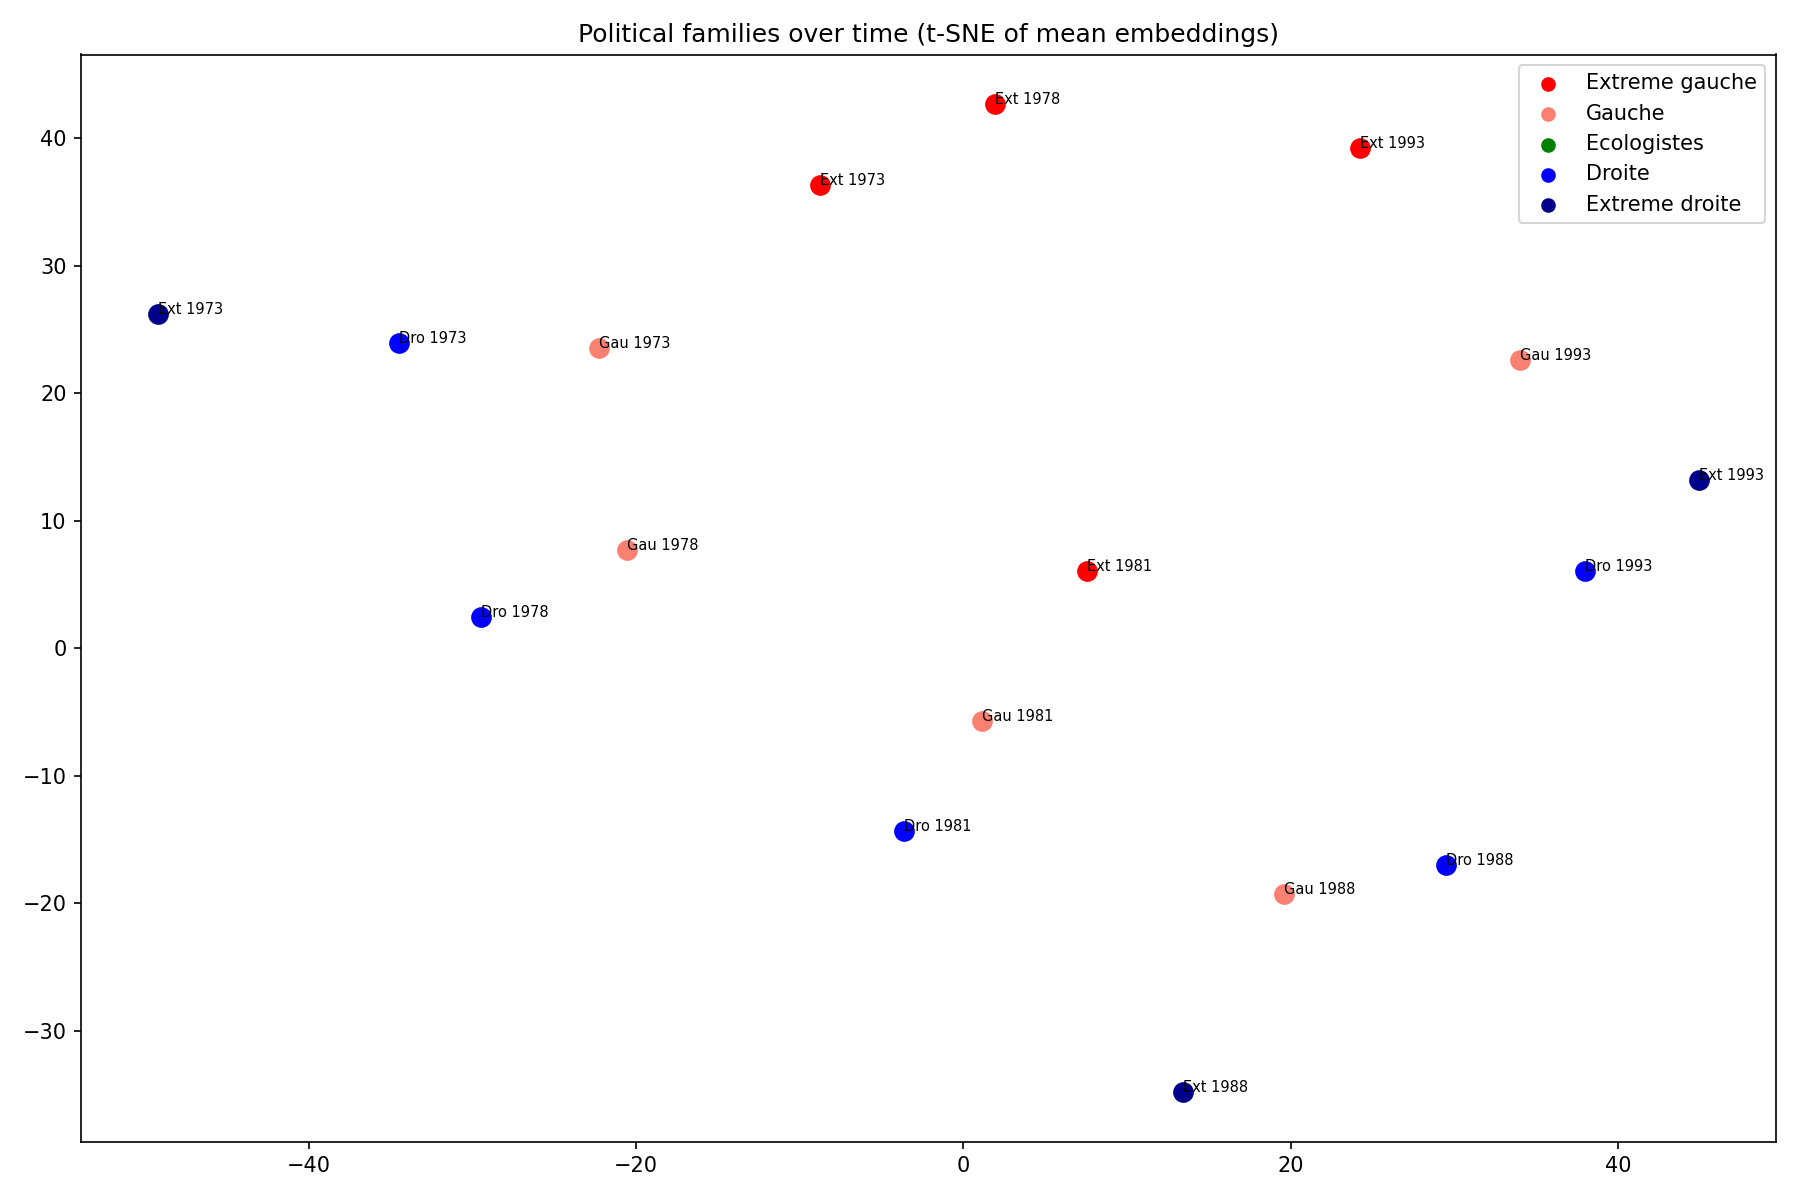
\includegraphics[width=0.9\linewidth]{tsne_temporal_evolution.png}
  \caption{t-SNE of mean embeddings per political family and election year. Labels are abbreviated: Dro = Droite, Ext = Extr\^{e}me gauche or Extr\^{e}me droite, Gau = Gauche, Eco = \'{E}cologistes. Low point count limits interpretability.}
  \label{fig:temporal}
\end{figure}

%----------------------------------------------------------------------
\section{Discussion}
\label{sec:discussion}
%----------------------------------------------------------------------

The main result is that TF-IDF with logistic regression reaches 84\% accuracy even after removing all explicit party names from the text. CamemBERT, despite being a much larger model, only gets to 71\%. We initially expected CamemBERT to be better, because it can capture contextual information that TF-IDF ignores. But in practice, the discriminative signal in \textit{professions de foi} seems to be mostly about which specific words are used, not about how they relate to each other in context. A simple bag-of-words is enough to pick up on that.

\paragraph{Why TF-IDF works so well.}
The feature analysis from Section~\ref{sec:results} helps explain this. Basically, the classifier picks up on a few keywords that are very specific to each political family. For example, Extr\^{e}me gauche texts use words like ``travailleurs'' or ``lutte'' that you almost never find in other families, and that is enough to get F1 = 0.96. \citet{laver2003extracting} showed something similar with their Wordscores method: just looking at word frequencies in political texts is enough to estimate where parties stand, even though their method puts parties on a continuous left-right scale instead of classifying them. Our results point in the same direction --- word-level features work well for this kind of task.

We also noticed that some of the top features are not really about political discourse. ``Le~Pen'' comes up as a strong feature for Extr\^{e}me droite because FN candidates often mention their leader, and we only clean party names, not people's names. ``communiste'' and ``gauche'' also stay in the text because we remove full names like ``Parti Communiste Fran\c{c}ais'' but not single words. We decided to keep it that way because these words are part of how candidates talk about their political identity --- it is not exactly data leakage, but it does help the model.

\paragraph{The Gauche--Droite confusion.}
The confusion matrix shows that 76 Gauche texts get predicted as Droite, and 12 the other way around. This is the biggest source of error. We think this makes sense if you consider the political context: during 1973--1993, France went through the \textit{alternance} of 1981 (first left-wing president) and then the \textit{cohabitation} periods. After these events, the PS and the mainstream right started using more and more similar language --- both talk about employment, housing, modernization, etc. So the fact that the classifier has trouble telling them apart is not that surprising, it actually reflects something real about how political discourse evolved.

The cosine similarity heatmap (Figure~\ref{fig:cosine}) shows the same thing. Most parties end up with similarity above 0.90, so their discourse is really quite close. The RPCR is the only real outlier (it is a party from New Caledonia with completely different concerns). We can also see that LO and PSU are a bit further from right-wing parties, which makes sense given their more radical positions.

For the embeddings, we first tried using CamemBERT base \texttt{[CLS]} tokens but it did not work at all --- cosine similarities were all above 0.98, so everything looked the same (see Appendix~\ref{app:cls_failure}). We had to switch to a sentence-transformer to get useful results.

\paragraph{Why CamemBERT underperforms.}
We think there are a few reasons. The dataset is small (3{,}163 training examples for 110M parameters), so the model overfits --- we can see it clearly in the training curves. But it is not just about data size. The signal in these texts is mostly about which words appear, not about how they relate to each other in context. TF-IDF captures that kind of signal just fine, so CamemBERT does not really add anything. On top of that, the 512-token limit hurts a lot: Extr\^{e}me gauche texts are around 6{,}700 words on average, so CamemBERT only sees the beginning. TF-IDF uses the whole text, which is a big advantage here.

\paragraph{Limitations.}
First, our regex labeling only works when the party name is written in the text. Left-wing parties like PCF or LO almost always state their name, but right-wing candidates often run under coalition labels or do not mention a party at all. This is why we have more left-wing than right-wing documents.

Second, as we mentioned, words like ``communiste'', ``gauche'', or ``Le~Pen'' are still in the cleaned text. We chose to only remove full party names, not individual political words, because they are part of how candidates express their views. But it means the classifier partly relies on these markers.

Third, the OCR quality is not the same across years. Older documents (1973, 1978) have more errors, and we did not try to correct them. It adds noise but we are not sure how much it matters in practice.

Fourth, CamemBERT only reads the first 512 tokens, so it misses most of the longer documents. We thought about chunking or hierarchical models but it seemed too complex for the potential gain. Also, the t-SNE plots should be read carefully --- t-SNE can distort distances, and the temporal plot (Figure~\ref{fig:temporal}) has only 18 points.

Finally, the big difference in text length between families (Table~\ref{tab:lengths}) means that TF-IDF partly captures length instead of content. A 6{,}000-word document will have higher scores for common words than a 1{,}000-word one, just because there are more words. We did not normalize for this, and it probably helps explain the good performance on Extr\^{e}me gauche.

%----------------------------------------------------------------------
\section{Conclusion}
\label{sec:conclusion}
%----------------------------------------------------------------------

Our main finding is that a TF-IDF logistic regression reaches 84\% accuracy at predicting political families from \textit{professions de foi}, even without any party name in the text. CamemBERT does not improve on this (71\%), which we attribute to the small dataset size, the lexical nature of the signal, and the 512-token truncation that is especially penalizing for the longest documents. The feature analysis showed that classification relies on distinctive political vocabulary (like ``travailleurs'' for the far left), but also on residual markers that our cleaning did not fully remove. The sentence-transformer analysis shows that party discourses are overall quite similar (cosine similarities above 0.90 for most pairs), though the extremes of the political spectrum are more distinctive.

Perhaps the most interesting result is the confusion between Gauche and Droite, which suggests a real convergence in mainstream political discourse during this period --- something that is well documented in political science but that we can observe here through a purely computational approach.

Several extensions would be natural. Matching candidates against electoral result databases could improve the labeling of right-wing parties and reduce class imbalance. It would also be interesting to apply the same approach to more recent elections, where party discourse may have diverged more, especially with the rise of new political movements.

\begin{ack}
This work was conducted as part of the NLP course at ENSAE Paris (2025--2026). We thank the Archelec project at Sciences Po for making the corpus available, and Christopher Kermorvant for providing the OCR'd text files.
\end{ack}

\bibliographystyle{plainnat}

\begin{thebibliography}{10}

\bibitem[Archelec()]{archelec}
Sciences~Po, CEVIPOF.
\newblock Archelec -- Archives \'{E}lectorales.
\newblock \url{https://archelec.sciencespo.fr}.


\bibitem[Laver et~al.(2003)]{laver2003extracting}
M.~Laver, K.~Benoit, and J.~Garry.
\newblock Extracting policy positions from political texts using words as data.
\newblock \emph{American Political Science Review}, 97(2):311--331, 2003.

\bibitem[Martin et~al.(2020)]{martin2020camembert}
L.~Martin, B.~Muller, P.~J.~Ortiz~Su\'{a}rez, Y.~Dupont, L.~Romary, E.~de~la~Clergerie, D.~Seddah, and B.~Sagot.
\newblock CamemBERT: a tasty French language model.
\newblock In \emph{Proceedings of ACL}, pages 7203--7219, 2020.

\bibitem[Rheault and Cochrane(2020)]{rheault2020word}
L.~Rheault and C.~Cochrane.
\newblock Word embeddings for the analysis of ideological placement in parliamentary corpora.
\newblock \emph{Political Analysis}, 28(1):112--133, 2020.

\bibitem[Volkens et~al.(2013)]{volkens2013manifesto}
A.~Volkens, P.~Lehmann, N.~Merz, S.~Regel, and A.~Werner.
\newblock The Manifesto Data Collection.
\newblock \emph{Manifesto Project (MRG/CMP/MARPOR)}, Version 2013a, 2013.

\end{thebibliography}

%%%%%%%%%%%%%%%%%%%%%%%%%%%%%%%%%%%%%%%%%%%%%%%%%%%%%%%%%%%%
\appendix

\section{Implementation details}
\label{app:implementation}

All code is available on GitHub\footnote{\url{https://github.com/MaelTremouille/political-text-classification}}. The pipeline described in Sections~\ref{sec:data}--\ref{sec:results} consists of four scripts:

\begin{enumerate}
    \item \texttt{data\_preparation.py}: parses raw text files, filters \textit{professions de foi}, aggregates multi-page documents, and produces a Parquet file.
    \item \texttt{label\_extraction.py}: extracts party labels via regex, removes party mentions from text, assigns political families, and creates stratified train/val/test splits.
    \item \texttt{classification.py}: trains the TF-IDF baseline and fine-tunes CamemBERT, evaluates both on the test set, and saves results.
    \item \texttt{political\_mapping.py}: extracts sentence-transformer embeddings, computes similarity matrices, and produces visualization figures.
\end{enumerate}

CamemBERT fine-tuning was performed on an Apple M-series chip (MPS backend). Each training epoch takes approximately 30 minutes.

\newpage
\section{CamemBERT training configurations}
\label{app:training}

As discussed in Section~\ref{sec:models}, we tested multiple CamemBERT configurations to improve performance:

\begin{itemize}
    \item \textbf{Without class weighting} (5 classes, 3 epochs): the model predicts the majority class (Gauche) for most inputs, achieving 75\% accuracy but 0\% recall on minority classes.
    \item \textbf{With class weighting} (5 classes, 3 epochs): weighted cross-entropy loss forces attention to minority classes, but \'{E}cologistes (weight $= 23.6\times$) destabilizes training. Test accuracy: 60\%.
    \item \textbf{4 classes, weighted, no scheduler} (3 epochs): removing \'{E}cologistes stabilizes training. Test accuracy: 68\%.
    \item \textbf{4 classes, weighted, with scheduler} (5 epochs): linear warmup and decay of learning rate. Test accuracy: 71\%. Overfitting observed from epoch 3 onward (training loss decreases while validation accuracy stagnates).
\end{itemize}

In all cases, the TF-IDF baseline (84\%) outperforms CamemBERT.

\newpage
\section{CamemBERT base embeddings}
\label{app:cls_failure}

As mentioned in Section~\ref{sec:mapping}, our initial approach for semantic mapping used the \texttt{[CLS]} token embedding from the pretrained (not fine-tuned) CamemBERT base model. We computed cosine similarity between mean embeddings per party and found that all pairwise similarities exceeded 0.98 (Figure~\ref{fig:cls_heatmap}). The resulting heatmap was uninformative: all parties appeared equally similar.

This is because CamemBERT base was trained for masked language modeling, not for producing sentence-level semantic representations. Its \texttt{[CLS]} token is not optimized for semantic similarity, and since all \textit{professions de foi} share a similar formal French register, their representations converge.

We addressed this by switching to a sentence-transformer model (\texttt{dangvantuan/sentence-camembert-large}) trained specifically for semantic similarity, which uses mean pooling over all tokens rather than the \texttt{[CLS]} token alone. The resulting heatmap (Figure~\ref{fig:cosine}) shows meaningful variation (0.70--1.00), validating this choice.

\begin{figure}[h]
  \centering
  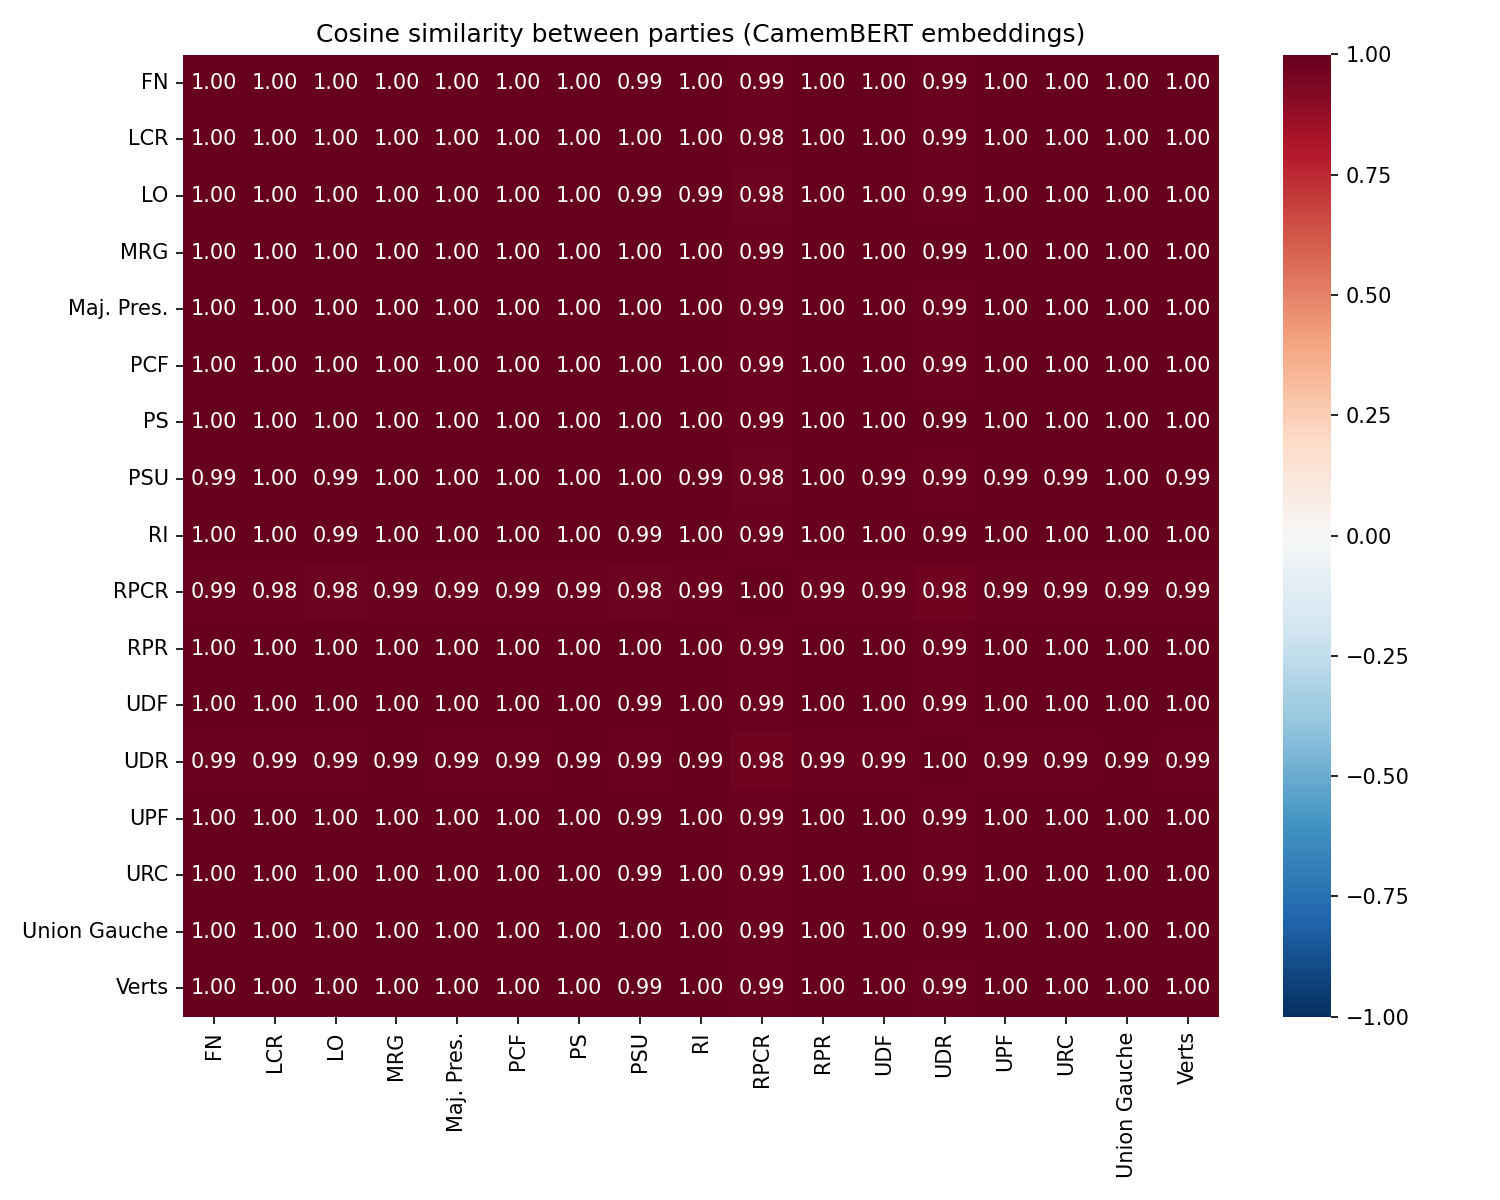
\includegraphics[width=0.75\linewidth]{cosine_similarity_parties_base.png}
  \caption{Cosine similarity between mean party embeddings using CamemBERT base \texttt{[CLS]} token. All values exceed 0.98, making the representation uninformative for discriminating parties.}
  \label{fig:cls_heatmap}
\end{figure}

\newpage
\section{Top 20 TF-IDF features per class}
\label{app:features}

Table~\ref{tab:top_features} shows the 20 features with the highest logistic regression coefficients for each political family. Recall that our TF-IDF vectorizer uses both unigrams (single words) and bigrams (pairs of consecutive words), so some features like ``les travailleurs'' or ``france unie'' are bigrams while ``travailleurs'' or ``notre'' are unigrams. A feature can therefore appear both as a unigram and as part of a bigram.

Several patterns are worth noting. First, many top features are dates (``12 juin'', ``28 mars'', ``mars 1973'') or geographic names (``guadeloupe'', ``la r\'{e}union'', ``metz'', ``nice''). These are not really political vocabulary --- they reflect when and where elections took place, and certain parties are more represented in certain years or departments. Second, we notice German words (``die'', ``und'') among Extr\^{e}me gauche features, which likely come from bilingual \textit{professions de foi} in Alsace. Third, ``immigration'' and ``fran\c{c}ais abord'' (\textit{French first}) for Extr\^{e}me droite, and ``travailleurs'' (\textit{workers}) for Extr\^{e}me gauche, are genuinely political terms that reflect each family's core ideology.

\begin{table}[h]
  \caption{Top 20 TF-IDF features per political family, ranked by logistic regression coefficient. Features can be unigrams or bigrams (marked with *).}
  \label{tab:top_features}
  \centering
  \small
  \begin{tabular}{rlrl}
    \toprule
    \multicolumn{2}{c}{\textbf{Extr\^{e}me gauche}} & \multicolumn{2}{c}{\textbf{Gauche}} \\
    Coef. & Feature & Coef. & Feature \\
    \midrule
    4.30 & les          & 1.92 & le \\
    3.06 & travailleurs & 1.59 & du \\
    3.02 & de           & 1.28 & la \\
    2.42 & des          & 1.15 & juin \\
    2.06 & il           & 1.00 & 19 mars* \\
    2.03 & ils          & 0.97 & politique \\
    1.97 & die          & 0.96 & dans \\
    1.74 & qu           & 0.94 & gauche \\
    1.44 & est          & 0.92 & communiste \\
    1.40 & les travailleurs* & 0.90 & une \\
    1.39 & que          & 0.86 & 19 \\
    1.28 & la           & 0.85 & maire \\
    1.26 & on           & 0.85 & candidat \\
    1.20 & mais         & 0.83 & 1973 \\
    1.18 & ans          & 0.81 & 1981 \\
    1.16 & pas          & 0.79 & de \\
    1.10 & und          & 0.79 & 11 mars* \\
    1.04 & voter        & 0.76 & juin 1981* \\
    1.01 & nous         & 0.75 & mars 1973* \\
    1.01 & ne           & 0.74 & majorit\'{e} \\
    \midrule
    \multicolumn{2}{c}{\textbf{Droite}} & \multicolumn{2}{c}{\textbf{Extr\^{e}me droite}} \\
    Coef. & Feature & Coef. & Feature \\
    \midrule
    1.73 & 12 juin*     & 2.29 & 28 mars* \\
    1.10 & la r\'{e}union* & 1.96 & 28 \\
    0.99 & juin 1988*   & 1.73 & metz \\
    0.99 & 1988         & 1.53 & nice \\
    0.93 & notre        & 1.43 & 1993 \\
    0.87 & guadeloupe   & 1.30 & le 28* \\
    0.85 & 28 mars*     & 1.26 & haute sa\^{o}ne* \\
    0.84 & france unie* & 1.23 & fran\c{c}ais \\
    0.83 & r\'{e}union  & 1.15 & mars 1993* \\
    0.82 & juin         & 1.14 & le pen* \\
    0.74 & corse        & 1.04 & pen \\
    0.70 & en appelle*  & 1.03 & saint denis* \\
    0.67 & du 12*       & 1.02 & cercle national* \\
    0.66 & unie         & 1.00 & limoges \\
    0.64 & solidarit\'{e} & 1.00 & de nice* \\
    0.64 & 12           & 0.98 & cercle \\
    0.63 & r\'{e}unionnais & 0.98 & fran\c{c}ais abord* \\
    0.63 & loir         & 0.98 & marie le* \\
    0.62 & je           & 0.96 & haute \\
    0.59 & \'{e}coute   & 0.95 & immigration \\
    \bottomrule
  \end{tabular}
\end{table}

%%%%%%%%%%%%%%%%%%%%%%%%%%%%%%%%%%%%%%%%%%%%%%%%%%%%%%%%%%%%

\newpage
\section*{NeurIPS Paper Checklist}

\begin{enumerate}

\item {\bf Claims}
    \item[] Question: Do the main claims made in the abstract and introduction accurately reflect the paper's contributions and scope?
    \item[] Answer: \answerYes{}
    \item[] Justification: The abstract and introduction state the four contributions: labelled dataset construction, a before/after lexical-cleaning comparison that exposes what TF-IDF actually classifies on, a data-efficient frozen sentence-CamemBERT head as a parameter-matched control, and a temporal-split evaluation with quantitative clustering metrics on the semantic map.

\item {\bf Limitations}
    \item[] Question: Does the paper discuss the limitations of the work performed by the authors?
    \item[] Answer: \answerYes{}
    \item[] Justification: Section~6 discusses residual candidate/toponym leakage after v2 cleaning, regex labelling bias, uneven OCR quality, the 512-token truncation in fine-tuned CamemBERT, the absence of continued masked-language-model pretraining, and the length bias between political families.

\item {\bf Theory assumptions and proofs}
    \item[] Answer: \answerNA{}
    \item[] Justification: This paper is empirical and does not include theoretical results.

\item {\bf Experimental result reproducibility}
    \item[] Answer: \answerYes{}
    \item[] Justification: All hyperparameters, data splits, and model choices are described. Code is provided in the GitHub repository.

\item {\bf Open access to data and code}
    \item[] Answer: \answerYes{}
    \item[] Justification: Code is available on GitHub. The corpus is publicly available through the Archelec project.

\item {\bf Experimental setting/details}
    \item[] Answer: \answerYes{}
    \item[] Justification: Section~4 details all training parameters (learning rate, batch size, epochs, optimizer, TF-IDF settings).

\item {\bf Experiment statistical significance}
    \item[] Answer: \answerYes{}
    \item[] Justification: TF-IDF and the frozen sentence-CamemBERT head are evaluated with 5-fold stratified cross-validation (mean $\pm$ s.d.\ reported) and with bootstrap 95\% confidence intervals on macro-F1 (1{,}000 resamples). Temporal generalisation is tested with three held-out-year splits (Table~7). CamemBERT fine-tuning uses a single seeded run because of training time.

\item {\bf Experiments compute resources}
    \item[] Answer: \answerYes{}
    \item[] Justification: Appendix~A reports the hardware used (Apple M-series, MPS backend) and approximate training times.

\item {\bf Code of ethics}
    \item[] Answer: \answerYes{}
    \item[] Justification: The research uses publicly available historical documents and does not raise ethical concerns.

\item {\bf Broader impacts}
    \item[] Answer: \answerNA{}
    \item[] Justification: This is an academic study of historical political texts with no direct deployment implications.

\item {\bf Safeguards}
    \item[] Answer: \answerNA{}
    \item[] Justification: The models are trained on public historical data and pose no misuse risk.

\item {\bf Licenses for existing assets}
    \item[] Answer: \answerYes{}
    \item[] Justification: The Archelec corpus is cited and its source URL provided. CamemBERT is cited with its original publication.

\item {\bf New assets}
    \item[] Answer: \answerNA{}
    \item[] Justification: No new datasets or models are released.

\item {\bf Crowdsourcing and research with human subjects}
    \item[] Answer: \answerNA{}
    \item[] Justification: No human subjects were involved.

\item {\bf Institutional review board (IRB) approvals or equivalent for research with human subjects}
    \item[] Answer: \answerNA{}
    \item[] Justification: No human subjects were involved.

\item {\bf Declaration of LLM usage}
    \item[] Answer: \answerNA{}
    \item[] Justification: No LLM is used as a component of the core methodology. CamemBERT is a pretrained encoder model fine-tuned for classification, not used as a generative LLM.

\end{enumerate}


\end{document}
